\documentclass{article}

\usepackage{fancyhdr}
\usepackage{extramarks}
\usepackage{amsmath}
\usepackage{amsthm}
\usepackage{amsfonts}
\usepackage{tikz}
\usepackage[plain]{algorithm}
\usepackage{algpseudocode}
\usepackage{listings}
\usepackage{xcolor}
\usepackage[english]{babel}
\usepackage[T1]{fontenc}
\usepackage{lmodern,mathrsfs}
\usepackage{xparse}
\usepackage[inline,shortlabels]{enumitem}
\setlist{topsep=2pt,itemsep=2pt,parsep=0pt,partopsep=0pt}
\usepackage[dvipsnames]{xcolor}
\usepackage[utf8]{inputenc}
\usepackage[a4paper,top=0.5in,bottom=0.2in,left=0.5in,right=0.5in,footskip=0.3in,includefoot]{geometry}
\usepackage[most]{tcolorbox}
\tcbuselibrary{minted} % tcolorbox minted library, required to use the "minted" tcb listing engine (this library is not loaded by the option [most])
\usepackage{minted} % Allows input of raw code, such as Python code
% \usepackage[colorlinks]{hyperref}


\usetikzlibrary{automata,positioning}

\tcbset{
    pythoncodebox/.style={
        enhanced jigsaw,breakable,
        colback=gray!10,colframe=gray!20!black,
        boxrule=1pt,top=2pt,bottom=2pt,left=2pt,right=2pt,
        sharp corners,before skip=10pt,after skip=10pt,
        attach boxed title to top left,
        boxed title style={empty,
            top=0pt,bottom=0pt,left=2pt,right=2pt,
            interior code={\fill[fill=tcbcolframe] (frame.south west)
                --([yshift=-4pt]frame.north west)
                to[out=90,in=180] ([xshift=4pt]frame.north west)
                --([xshift=-8pt]frame.north east)
                to[out=0,in=180] ([xshift=16pt]frame.south east)
                --cycle;
            }
        },
        title={#1}, % Argument of pythoncodebox specifies the title
        fonttitle=\sffamily\bfseries
    },
    pythoncodebox/.default={}, % Default is No title
    %%% Starred version has no frame %%%
    pythoncodebox*/.style={
        enhanced jigsaw,breakable,
        colback=gray!10,coltitle=gray!20!black,colbacktitle=tcbcolback,
        frame hidden,
        top=2pt,bottom=2pt,left=2pt,right=2pt,
        sharp corners,before skip=10pt,after skip=10pt,
        attach boxed title to top text left={yshift=-1mm},
        boxed title style={empty,
            top=0pt,bottom=0pt,left=2pt,right=2pt,
            interior code={\fill[fill=tcbcolback] (interior.south west)
                --([yshift=-4pt]interior.north west)
                to[out=90,in=180] ([xshift=4pt]interior.north west)
                --([xshift=-8pt]interior.north east)
                to[out=0,in=180] ([xshift=16pt]interior.south east)
                --cycle;
            }
        },
        title={#1}, % Argument of pythoncodebox specifies the title
        fonttitle=\sffamily\bfseries
    },
    pythoncodebox*/.default={}, % Default is No title
}

% Custom tcolorbox for Python code (not the code itself, just the box it appears in)
\newtcolorbox{pythonbox}[1][]{pythoncodebox=#1}
\newtcolorbox{pythonbox*}[1][]{pythoncodebox*=#1} % Starred version has no frame

\tcbset{
    rcodebox/.style={
        enhanced jigsaw,breakable,
        colback=blue!5,colframe=blue!40!black,
        boxrule=1pt,top=2pt,bottom=2pt,left=2pt,right=2pt,
        sharp corners,before skip=10pt,after skip=10pt,
        attach boxed title to top left,
        boxed title style={empty,
            top=0pt,bottom=0pt,left=2pt,right=2pt,
            interior code={\fill[fill=tcbcolframe] (frame.south west)
                --([yshift=-4pt]frame.north west)
                to[out=90,in=180] ([xshift=4pt]frame.north west)
                --([xshift=-8pt]frame.north east)
                to[out=0,in=180] ([xshift=16pt]frame.south east)
                --cycle;
            }
        },
        title={#1},
        fonttitle=\sffamily\bfseries
    },
    rcodebox/.default={}, % Default title = none
    % Starred version has no frame
    rcodebox*/.style={
        enhanced jigsaw,breakable,
        colback=blue!5,coltitle=blue!40!black,colbacktitle=tcbcolback,
        frame hidden,
        top=2pt,bottom=2pt,left=2pt,right=2pt,
        sharp corners,before skip=10pt,after skip=10pt,
        attach boxed title to top text left={yshift=-1mm},
        boxed title style={empty,
            top=0pt,bottom=0pt,left=2pt,right=2pt,
            interior code={\fill[fill=tcbcolback] (interior.south west)
                --([yshift=-4pt]interior.north west)
                to[out=90,in=180] ([xshift=4pt]interior.north west)
                --([xshift=-8pt]interior.north east)
                to[out=0,in=180] ([xshift=16pt]interior.south east)
                --cycle;
            }
        },
        title={#1},
        fonttitle=\sffamily\bfseries
    },
    rcodebox*/.default={}, % Default title = none
}

% Custom tcolorbox environments
\newtcolorbox{rbox}[1][]{rcodebox=#1}
\newtcolorbox{rbox*}[1][]{rcodebox*=#1}

% Basic Document Settings
\topmargin=-0.45in
\evensidemargin=0in
\oddsidemargin=0in
\textwidth=6.5in
\textheight=9.0in
\headsep=0.25in
\linespread{1.1}

\pagestyle{fancy}
\lhead{\hmwkAuthorName}
\chead{\hmwkClass\ (\hmwkClassInstructor): \hmwkTitle}
\rhead{\firstxmark}
\lfoot{\lastxmark}
\cfoot{\thepage}
\renewcommand\headrulewidth{0.4pt}
\renewcommand\footrulewidth{0.4pt}
\setlength\parindent{0pt}

% Homework Details
\newcommand{\hmwkTitle}{Examen 3}
\newcommand{\hmwkDueDate}{Mayo 12, 2025}
\newcommand{\hmwkClass}{ESMA 6787}
\newcommand{\hmwkClassInstructor}{Damaris Santana}
\newcommand{\hmwkAuthorName}{\textbf{Alejandro Ouslan}}

% Title Page
\title{
	\vspace{2in}
	\textmd{\textbf{\hmwkClass:\ \hmwkTitle}}\\
	\normalsize\vspace{0.1in}\small{Due\ on\ \hmwkDueDate}\\
	\vspace{0.1in}\large{\textit{\hmwkClassInstructor}}
	\vspace{3in}
}

\author{\hmwkAuthorName}
\date{}


% Begin document
\begin{document}
\maketitle
\pagebreak
\tableofcontents
\pagebreak

% Homework problem 1
\section{problem 1}
Define using your own words:
\begin{enumerate}
	\item Estimate $c'\beta$
	\item Power
	\item Null hypothesis
	\item Alternative hypothesis
	\item Test Statistics
	\item Non-centrality parameter
	\item Details about the non-centrality parameter
\end{enumerate}

% Homework problem 2
\section{Problem 2}
Consider a completely randomized design with four treatment groups, with $n_i>0$ units assigned to treatment $i=1,2,3,4$.
\begin{enumerate}
	\item One way to model data from such an experiment is with the effect model:
	      $$
		      y_{ij}=\alpha + \tau_i + \epsilon{ij}, \quad i=1,2,3,4; \quad j= 1.\ldots, n_i
	      $$
	      Under this model show why each of the following is estimable or nonestimable:
	      $$
		      \tau_3, \tau_3 - \tau_2, \tau_3 + \tau_2
	      $$
	\item Now define a different model for the same experiment, as:
	      $$
		      y_{1j}= \mu_1 + \epsilon_{1j}, \quad j=1,\ldots,n_i
	      $$
	      $$
		      y_{ij}= \mu_1 + \theta_i + \epsilon_{ij} \quad i=2,3,4; \quad j=1,\ldots,n_i
	      $$
	      Under this model, show why each of the followings is estimable or nonestimable:
	      $$
		      \theta_3,\theta_3-\theta_2, \theta_3 + \theta_2
	      $$
\end{enumerate}

% Homework problem 3
\section{problem 3}

A chemical engineer is interested in comparing three different versions of a reaction process, labeled
A, B, and C, with respect to “percent conversion of feedstock.” In a preliminary experiment, she
applied each process to four batches of raw material, using appropriate randomization of the 12
available batches to the three treatments, and collected the percent conversion values presented in
the following table.

$$
	\begin{array}{|c|c|c|}
		\hline
		A    & B    & C    \\
		\hline
		27.3 & 41.9 & 36.8 \\
		31.6 & 36.8 & 39.2 \\
		34.6 & 38.9 & 36.1 \\
		29.4 & 37.5 & 38.0 \\
		\hline
	\end{array}
$$

Assuming the data are independent and can be reasonably modeled as:
$$
	y_{ij}= \mu_i + \epsilon{ij}, \quad E(e_{ij})=0, \quad Var(e_{ij})= \sigma^2
$$
\begin{enumerate}
	\item Estimate $\sigma^2$ and test the hypothesis: $\mu_i = \mu_2 = \mu_3$ against $H_1$: at least one of $\mu_i$ is different.
	\item Using your estimate of $\sigma$ as if it were the true parameter value, how large would a follow-up experiment
	      (with equal sample sizes) have to be so that the $0.05$-level confidence interval for $\mu_1 - \mu_3$ would have expected width ($5\%$).
\end{enumerate}


% Homework problem 4
\section{problem 4}
Consider a completely randomized design with five treatment groups, in which a total of $N = 50$
units are to be used. Although it won’t be explicitly used in the analysis model, treatments $1$
through $5$ actually represent increasing concentrations of one component in an otherwise standard
chemical compound, and the primary purpose of the experiment is to understand whether certain
measurable properties of the compound change with this concentration. The investigator decides
to address these questions by estimating four quantities:
$$
	\tau_2 - \tau_1,\tau_3-\tau_2,\tau_4-\tau_3,\tau_5-\tau_4
$$
where each $\tau_i$ is a parameter in the standard effects model. Find the optimal allocation for the $50$
available units (i.e., values for $n_1,\ldots , n_5$) that minimizes the average variance of estimates of the
four contrasts of interest. Do this as a constrained, continuous optimization problem, then round
the solution to integer values that are consistent with the required constraint.

% Homework problem 5
\section{problem 5}
Continue working with the experimental design described in problem 2. Suppose the experiment-
specific treatment means in this problem, as would be expressed in the cell means model, are
actually:
$$
	\begin{array}{|c|c|c|c|c|}
		\hline
		\mu_1 & \mu_2 & \mu_3 & \mu_4 & \mu_5 \\
		\hline
		10    & 11    & 12    & 12    & 12    \\
		\hline
	\end{array}
$$
and $\sigma=2$. What is the power of the standard F-test for the hypothesis
$$
	\tau_1 = \tau_2 = \tau_3 = \tau_4 = \tau_5
$$
at $\alpha=0.05$:
\begin{enumerate}
	\item if all $n_i=10$?
	\item under the optimal sample sample allocation you found in problem 2?
	\item Derive an optimal allocation for the F-test of equal treatment effects, i.e, the sample size
	      (totaling 50) that would result in the greatest power, if in reality the experiment-specific means are
	      $\mu_1=10$ and $\tau_2 = \tau_3 = \tau_4 = \tau_5 =8$
\end{enumerate}

% Homework problem 6
\section{problem 6}
The entire class of ESMA 6616 wanted to study how the power of the F changes with the non-
centrality parameter $\lambda^2$. To achieve this we will do as follow. Consider the model
$$
	y_{ij} = \mu_i + \epsilon_{ij}
$$
Where $\epsilon_{ij}\sim N(0,\sigma^2)$, with $i=1,\ldots,k$ and $j=1,...,n_i$.

The null and alternative hypotheses for the ANOVA F-test are
\[
	\begin{split}
		H_0 & : \mu_1 = \ldots = \mu_k           \\
		H_1 & : \text{at least one is different}
	\end{split}
\]
The test rejects $H_0$ if the $F^\star$-statistic, defined as $F^\star = \frac{MS_{model}}{MS_{error}}$ , exceeds
a critical value.

The power of the ANOVA F-test, which measures the probability of rejecting $H_0$ when $H_1$ is true, is
given by $P(F^\star > \alpha|H_1)$. To calculate the power, we must know the distribution
of $F\star$. Under $H_0$, $F^\star \sim F_{k-1,\sum_{k}^{i=1}n_i-k}$
degrees of freedom. The distribution under $H_1$ depends on
the true differences among the group means.

Consider the following example $k = 5$ treatment groups with group sizes $n_1 = n_2 = n_3 = 10, n_4 = 8$,
and $n_5 = 6$. Further, assume the standard deviation $\sigma = 1.5$. The task is to find the power of the
test when $H_1$ is true, given the group means $\mu_1 = 2, \mu_2 = 3, \mu_3 = 2.5, \mu_4 = 0$, and $\mu_5 = 1$. Assume
we are using a significance level of 0.05.

The overall mean is defined $\bar{\mu}= \sum_{5}^{i=1}n_i*\frac{\mu_i}{\sum_{5}^{i=1}*n_i}$

The non-centrality parameter is $\frac{\sum_{5}^{i=1}n_i(\mu_i-\bar{\mu})^2}{\sigma^2}$

In R, the argument ncp stands for the non-centrality parameter in the desity functions. In this example, the test statisic
have the following distribution $F^\star \sim F_{5-1,40-5}(\lambda^2=0)$ under $H_0$ and $F^\star \sim F_{5-1,40-5}(\lambda^2 = 15.32222)$ under $H_1$.

Figure 1 showed the difference between the F distribution under the null hypothesis(solid red) with
4 and 35 with non-centrality parameter of 0 and the F under the alternative (dashed blue) with
the same degrees of freedom but non-centrality parameter $\lambda^2 = 15.3222$. We can observed as $\lambda^2$
increases the density under the alternative get farther from the null. The critical value to reject $H_0$
keeping the significance level $2.6415$. If $H_1$ is true and $F^\star \sim F_{5-1,40-5}(\lambda^2 = 15.32222)$, the power
to reject $H_0$ is the
$$
	P(F^\star>F_{k-1,\sum_{i=1}^{k}n_i-k,\alpha}|H_1)=0.8489175
$$
To interpret this value, the probability of rejecting the null hypothesis (non difference across the
means) when in fact there’s difference across the means is $0.8489$. To compute the critical value
and the power in R you can do the following,

\begin{figure}[H]
	\centering
	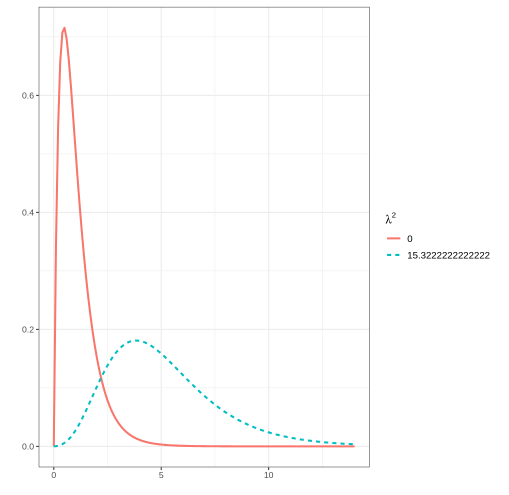
\includegraphics[width=0.5\textwidth]{assets/prob6.png}
	\caption{Comparison of the central (solid red) and non-central (dashed blue) $F$-distribution.}
\end{figure}

\begin{enumerate}
	\item Calculate the overall mean.
	\item Calculate the non-centrality parameter. Hint: The non-centrality parameter
	      should be a function of $n$.
	\item Find the critical value at the $5\%$ level. Note that the degrees of freedom should be a function of the
	      sample size $n$ as well.
	\item Compute the power for each sample size $n$, i.e., $n=2,3,4,\ldots,n_{min}$
	      where $n{min}$ is the minimum sample size such that power $\ge 0.95$.
	\item Use the following code to show your figure. This code will create the smae figure in this document, but you
	      must modify it to include your information.
\end{enumerate}

\begin{rbox}[Example Code]
	\inputminted{r}{code/prob6.R}
\end{rbox}

% Homework problem 7
\section{problem 7}
The entire class of ESMA 6616 wanted to study how the power of the F -test changes with the
non-centrality parameter $\lambda^2$. To achieve this, we will proceed as follows. Consider the model
$$
	y_{ij}= \mu_i + \epsilon_{ij}
$$
where $e{ij} \sim N(0,\sigma^2)$ with $i=1,\ldots,k$ and $j=1,\ldots,n_i$.
The null and alternative hypotheses for the ANOVA $F$-test are
$$
	H_0:\mu_i=\cdots=\mu_k \quad H_1: \text{at least one  $\mu_i$ is different}
$$
The test rejects $H_0$ if the statistic
$$
	F^\star = \frac{MS_{model}}{MS_{error}}
$$
exceeds a critical value.
The power of the ANOVA F -test, which measures the probability of rejecting H0 when H1 is true,
is given by
$$
	P(F^\star>\text{crtitical value}| H_1)
$$
To calculate the power, we must know the distribution of $F^\star$. Under $H_0$, we have
$$
	F^\star \sim F_{k-1,\sum_{i=1}^{k}n_i-k}
$$
The distribution under $H_1$ depends on the true differences among the group means.
Example: Consider $k = 5$ treatment groups with sample sizes $n_1 = n_2 = n_3 = 10, n_4 = 8$, and
$n_5 = 6$. Assume the standard deviation $\sigma = 1.5$. The task is to find the power of the test when $H_1$
is true, given the group means
$$
	\mu_1 = 2, \mu_2 = 3, \mu_3 = 2.5, \mu_4 =0, \mu_5 = 1
$$
with a significance level $\alpha = 0.05$
\begin{enumerate}
	\item Calculate the overall mean.
	\item Calculate the non-centrality parameter. (Note: it should be a function of $n$).
	\item Find the critical value at the $5\%$ level. Note that the degrees of freedom should be a function of the
	      sample size $n$ as well.
	\item Compute the power for each sample size $n$, i.e., $n=2,3,4,\ldots,n_{min}$
	      where $n{min}$ is the minimum sample size such that power $\ge 0.95$.
	\item se the provided R code to produce your figure. Modify the code to include your information
\end{enumerate}
\end{document}
